\documentclass{my_cv}

\usepackage{graphicX}
\usepackage[margin=0.5in]{geometry}

\usepackage{tikz}




\begin{document}


%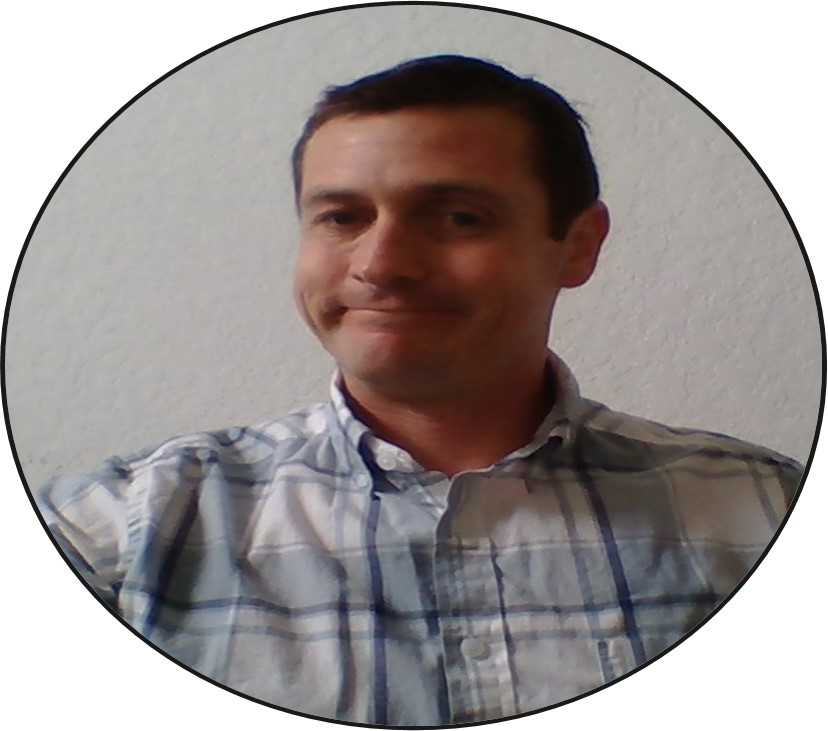
\includegraphics[width=5cm,height=5cm, keepaspectratio]{./images/resumepic.jpg}
\head{Adam Conn}{10965 Barbados Way}{San Diego}{CA}{92126}{aconn7395@gmail.com}{(619) 792-8677}
\vspace{.25in}

%\tikz[remember picture,overlay] \node[opacity=0.3,inner sep=0pt] at (current page.center){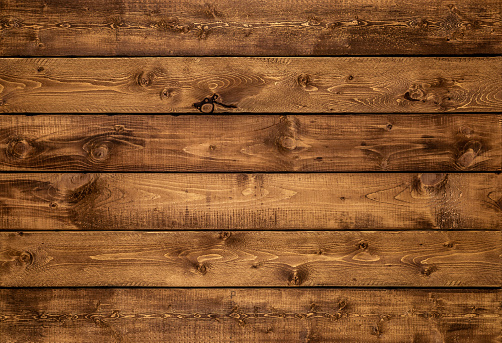
\includegraphics[width=\paperwidth,height=\paperheight]{images/bg.jpg}};

%The following is the skills page, there is really no good way to generalize it with my knowledge
\vspace{.25in}
\section{\huge{Skills}}
\textbf{Programming Languages:}
\begin{tabular}{ l @{ \textperiodcentered{ }}  l @{ \textperiodcentered{ }}l@{ \textperiodcentered{ }} l@{ \textperiodcentered{ }} l@{ \textperiodcentered{ }} l}
  python & java & c++ & HTML & CSS & Matlab \\

\end{tabular}
\tikz[remember picture,overlay] \node[opacity=0.3,inner sep=0pt] at (current page.center){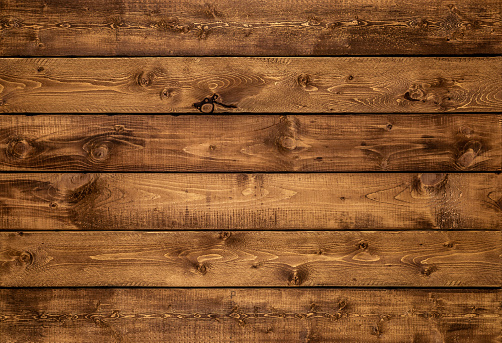
\includegraphics[width=\paperwidth,height=\paperheight]{images/bg.jpg}};

\vspace{.15in}
\noindent
\textbf{Frameworks/Libraries:}
\begin{tabular}{l@{ \textperiodcentered{ }} l @{ \textperiodcentered{ }}l @{ \textperiodcentered{ }}l@{ \textperiodcentered{ }} l@{ \textperiodcentered{ }} l}
  Django & matplotlib & numpy & sklearn & Bootstrap & JQuery\\
\end{tabular}

\vspace{0.15in}
\noindent
\textbf{Operating Systems:}
\begin{tabular}{l @{ \textperiodcentered{ }}l @{ \textperiodcentered{ }}l}
  Windows 8 & Mac OS & Linux/Unix\\
\end{tabular}

\vspace{0.15in}
\noindent
\textbf{Other:}

\vspace{.15in}
\begin{tabular}{ l @{ \textperiodcentered{ }}l @{ \textperiodcentered{ }}l @{ \textperiodcentered{ }}l}
  Linear Algebra & Probability & Basic Design Patterns & La\TeX \\
   Data Structures & Next-gen Sequencing & Protein Purification & RNA-Seq \\

\end{tabular}

\vspace{0.15in}
\noindent
\textbf{Algorithmic Knowledge:}

\vspace{.15in}
\begin{tabular}{@{ \textperiodcentered{}}l @{ \textperiodcentered{ }} l @{ \textperiodcentered{ }}l }
  \textbf{Machine Learning} & \textbf{General} & \textbf{Bioinformatics}\\
  \hline
  Linear Regression & Divide and Conquer &  Sequence Alignment\\
  Logistic Regression &   Greedy & Pairwise Alignment\\
  Support Vector Machines & Dynamic Programming &  Genome Assembly\\
  Neural Networks &  Recursive &  Motif Finding\\
  Decision Trees/Random Forest & Breadth First Search &  Gene Expression Analysis\\
  Hidden Markov Models &  Depth First Search & Gene Finding\\
  Boosting/Bagging Methods & Breadth First Search \\
  PCA & Djikstras \\
\end{tabular}

\section{Education}
\datedsubsection{University of California, San Diego}{2015}
B.S. in Bioengineering: Bioinformatics (3.5 GPA)
\datedsubsection{San Diego City College}{2012}
A.A. in Physics (3.9 GPA)



\newpage

\section{Work Experience}
%\datedsubsection{The Salk Institute}{Oct 2015 - Current}
\salk{images/salk}{Oct 2015 - Current}
\workitems{Collect data using high tech 3D laser scanning to capture the architect and
            morphology of a plant down to micrometer precision in the form of 3D
            coordinate point clouds.}
\workitems{ Design and write machine learning algorithms to find patterns within
            the 3D point cloud data.}
\workitems{ Write programs to visually view data using matplotlib.}
\workitems{ Implement statistical models that approximate and predict the intricate branching
            structures plants undergo as a response to a specific stressful environment.}
\workitems{ Built an automated pipeline to analyze RNA-SEQ datasets. Involved querying and
            downloading data from NCBI GEO by FTP, normalizing the data, building a binary classifier,
            and extracting the features (genes) used to build our classifier for future research.}
\workitems{ Attend presentations, collaborate with other departments and
           institutions, present work, and write sections of articles to
           be submitted for publication.}


%\datedsubsection{ Molecular Throughput inc.}{2009-2013}
\vspace{.25in}
\mtibio{images/mtibio_logo}{2009-2013}
\workitems{Directly responsible for purifying native and recombinant proteins.}
\workitems{Routinely worked with multiple cell lines (bacteria/insect/mammalian) to
            maintain, transform/transfect, ferment and harvest cells.}
\workitems{Created novel cDNA libraries.}
\workitems{Performed a wide variety of assays including PCR, RT-PCR, SDS-PAGE,
          western blots, DNA-agarose gel electrophoresis, nickel/ion-exchange/size
          exclusion chromatography, cell toxicology and enzyme kinetic assays.}



%\section{Education}
%\datedsubsection{University of California, San Diego}
%I attended the UCSD

%\section{Work}

%\datedsubsection{Salk}{2004--2008}
%  \workitems
%  {Point Clouds}
%  {Machine Learning}
%  {Other stuff}

\end{document}
